

To measure the $^{20}$F beta decay spectrum, a beam of $^{20}$F was implanted into one of two different detectors.
The isotope was implanted deeply enough from so that the detector material could completely absorb the energy of electron at the end point energy.
The implantation of the beam was done to avoid instrumental effects of a non-calorimetry experiment.
If there is a dead layer, there is more detector behind the layer to absorb the energy.
The electron cannot scatter out of the detector.

The experiment was run at the National Superconducting Cyclotron Laboratory (NSCL) in East Lansing, Michigan. 
The detector set up is describe below.

\section{Detector Set Up}

\subsection{$^{20}$F Decay Detectors}
One scintillator was a 3 in diameter by 3 in long cylinder of EJ-200 polyvinyltoluene (PVT).
It was attached to a clear plastic disk attached to a photomultiplier tube.
The idea was to avoid a rate dependent gain effect that was seen in a previous experiment.
The plastic detector signal is fast (around 100 ns) which makes pile-up a lesser concern.
This detector was built by colaborators for this experiment.
During the experiment the voltage on the PMT of this scintillator was varied.
This was due do an observed distortion in the beta decay spectrum.
A gain montitoring system was installed.

To monitor the gain of the plastic detector, a plastic disk containing an optical fiber was placed between the crystal and the photomultiplier tube. 
The other end of the fiber was fed into a box with an LED driven by a function generator. 
The box was made light-tight with electrical tape and black paint.
An additional optical fiber fed the light to a Si PIN diode.
This was to monitor the light output of the LED.

To help check for systematics effects, another implant detector was used.
It was a 2 in by 2 in by 4 in  CsI(Na) detector. 
This detector was a module from the CAESAR array \cite{Wei10}.
It does not have any gain monitoring like the PVT detector, but it is similar to a detector used in a different experiment. 
The other experiment was a similar measurement with $^{6}$He instead of $^{20}$F.

In order to measure the gamma ray from the $^{20}$F decay, a frame was built to hold four cubic 3 in CsI(Na) detectors.  
These were also part of the CAESAR array.
The frame to hold the four detectors was designed to be able to move the four outer detectors around in various configurations.
However, no other configurations were used during the experiment. 

A sketch of both detector configurations is shown in Figure \ref{fig:detsketch}.

\begin{figure}
	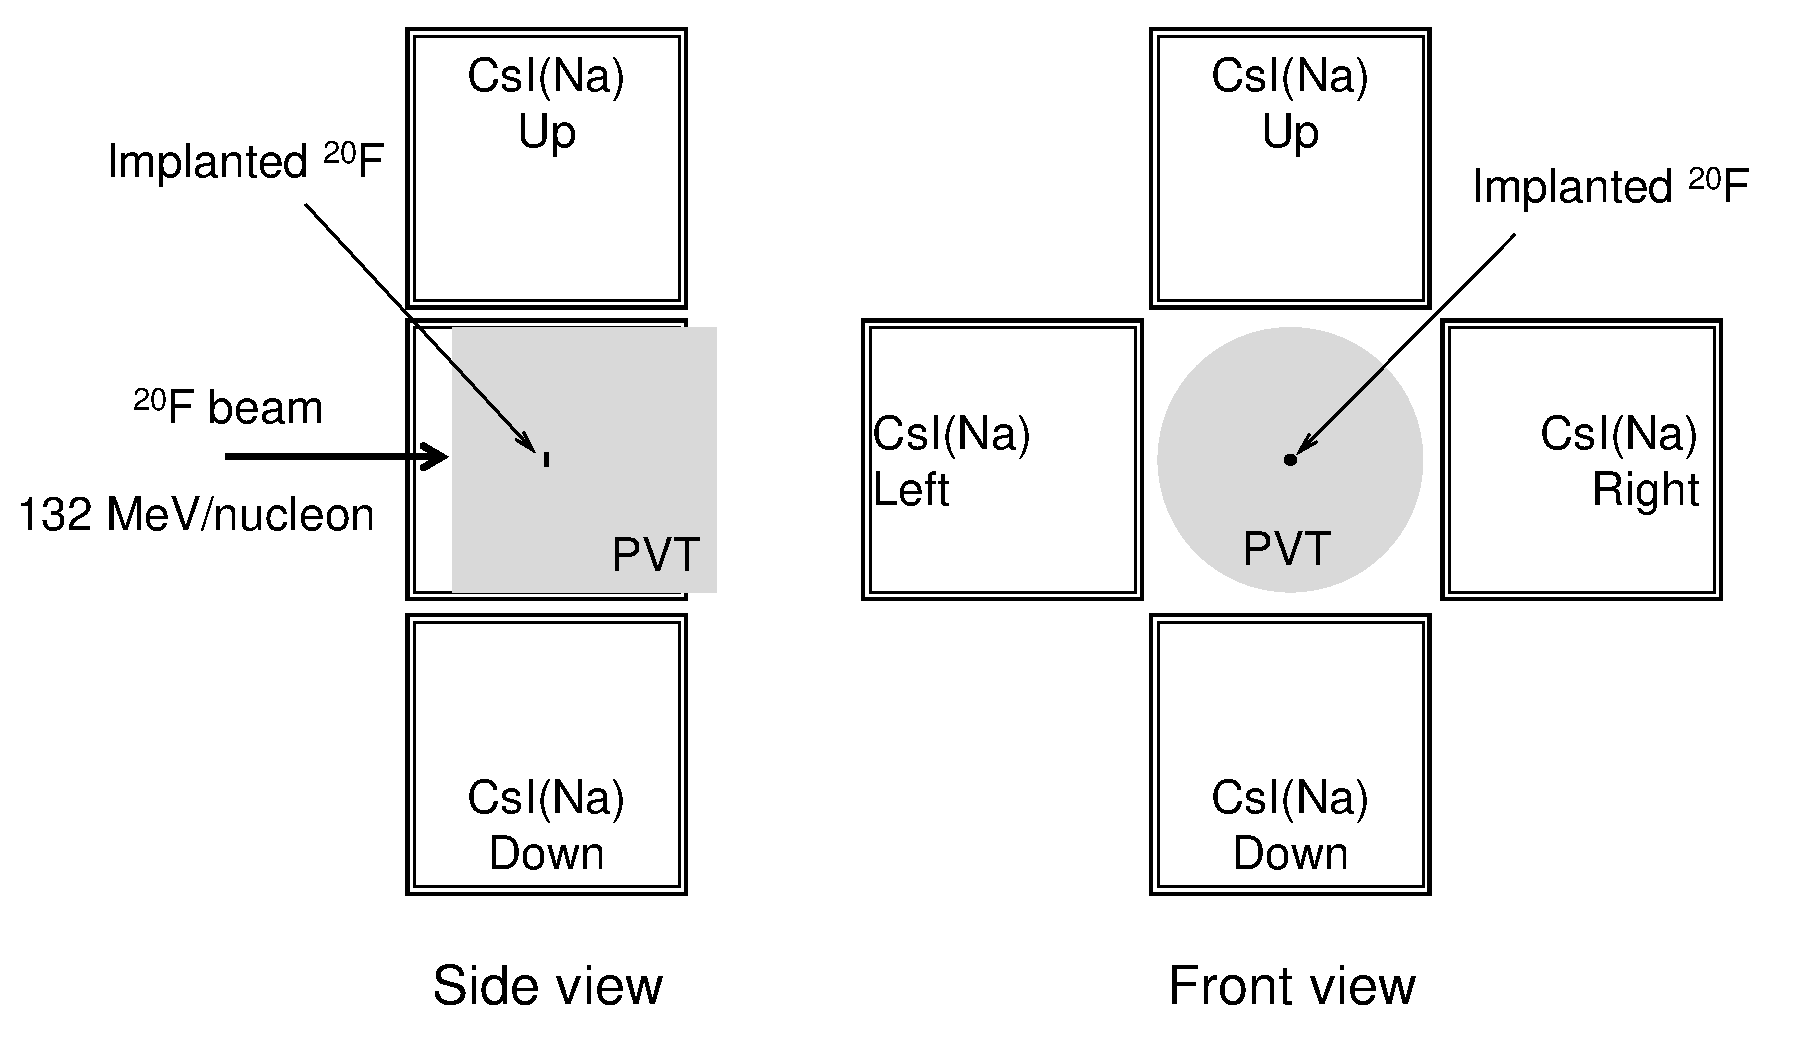
\includegraphics[width=0.88\textwidth]{fig_setup.pdf}
	\caption{A sketch of the detector set up. 
	Shown here is with the PVT detector implant.
	The CsI (Na) detector was centered in the middle of the the four gamma detectors and recessed by 1 inch.
	The bottom image shows a side of the detector set-up.}
	\label{fig:detsketch}
\end{figure}

To switch between different implant detectors, the central detector in the frame was removed and put on the floor.
The other detector was placed in the center of the four gamma detectors.
The PVT detector was supported on a metal rail, while the CsI (Na) detector was supported on pile of scrap aluminum.
Both of the detectors had the active scintillator part free in between the four large gamma detectors. 

\subsection{Other detectors}

The light from the LED was also piped to a PIN diode.
This was to get an independent measure of the light from the LEDs.
A parrallel plate avalanch counter (PPAC) was used for beams size measurements.
A Si detector was used to check the beam purity.
A pulser was used to make sure the data acquisition clock was stable.

\subsection{Powering the Detectors}

To power the gamma and implant scintillators, 3 2-channel NHQ 212M ISEG power supplies were used.
The Si detector was powered by a Tennelec TC248 amplifier.
The PPAC was powered by an integrated power supply.

Each detector had a different voltage. 
The PVT implant detector was varied in voltage over the course of the experiment.
This was due to concerns about saturation effects.
Initially, the high voltage on the PVT detector was chosen to take advantage of the dynamic range of the detector.
For the PPAC, 
The voltage for the four gamma detectors was chosen so that they had roughly the same gain.
The voltages of the detectors is shown in table \ref{tab:detvolt}.
\begin{table}[!hbt]
	\centering
		\begin{tabular}{r|l}
		Detector & HV (V) \\ \hline
		PVT Implant (Sets 1-4) & -975 \\
		PVT Implant (Set 5) & -856 \\
		PVT Implant (Set 6) & -780 \\
		CsI (Na) Implant & 780 \\ 
		CsI (Na) Gamma 1 & 930 \\
		CsI (Na) Gamma 2 & 1000 \\
		CsI (Na) Gamma 3 & 970 \\
		CsI (Na) Gamma 4 & 1015 \\
		Si Pin & 20 \\
		Pin diode & 15 \\
		PPAC & 560 
		\label{tab:detvolt}
		\end{tabular}
\end{table}

\section{Beam}

\subsection{Beam Discription}
The primary beam of $^{22}$Ne was accelerated by the coupled cyclotrons to 150 MeV/A. 
A typical intensity of the primary beam was around $60 * 10^{-5}$pnA.
It was impinged on a Be target and sent through the fragment separator. 
The resulting $^{20}$F beam was at an energy of 130 MeV/A. 
The intensity of the $^{20}$F was about $2 * 10^{-5}$ pnA, and the purity was about $93\%$ at the end of the fragment separator.

\subsection{Beam Size and Location}
To test the size of the beam, a parralel plate avalanche counter was used.
The size of the detector was 10 cm by 10 cm square. 
It was placed 65 cm upstream of the target.
A horizontal and verticle grid was in the detector.
Depending on where on each of the grids the particles hit, different charges were sent to either end of the PPAC.
The signals were fed into a digital data acquisition system, and read out as an energy.
The difference of the two signals divided by the sum was interpretted as a position.

To calibrate the detector, a mask with several holes was used. 
This mask covered the front of the detector, and an alpha source in the vacuum was placed in front of the PPAC.
Then, everything was left to run until an image of the mask was formed.
The mask had holes in it every 1 cm. 
It also had a large L shaped hole so that the orientation of the mask could be seen. 
With this, the PPAC could be calibrated.

Before taking data for the beta decay spectrum measurement, the PPAC was inserted into the beam.
After adjusting the parameters of the upstream beam optics, the final beam size at the PPAC was measured.
The calibrated data of the signals was built into a 3-D histogram.
There was some ringing in the PPAC, so the peak of the beam spot was fitted with a 3-D gaussian function.
The average of the gaussian and the sigma in the x and y direction was taken. 
From the sigmas, the half widths at half maximum (HWHM) in both directions were calculated. 
The distribution of the locations were sampled at eight different points. 
The points are shown as the black dots in Fig: \ref{fig:PPACSpotch}.
They are one HWHM away from the center. 

\begin{figure}
	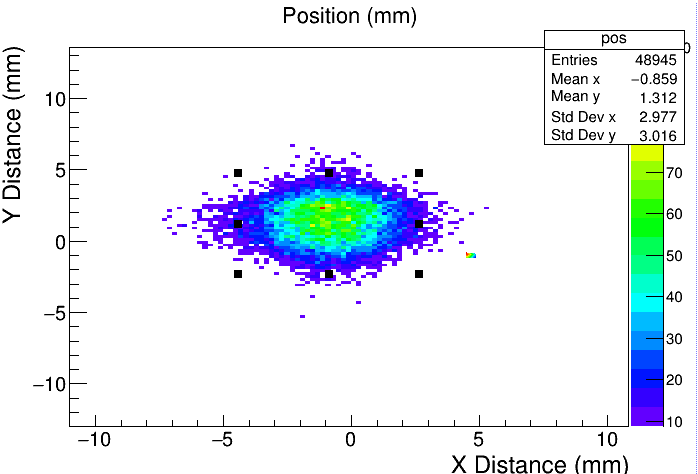
\includegraphics[width=0.88\textwidth]{PPACFitted.png}
	\caption{The beam spot of the calibrated PPAC spectrum. 
		 The samples of the spectrum that were averaged together are shown in the black dots.
		 The center of the fit is not shown.}
	\label{fig:PPACSpotch}
\end{figure}  

After averaging the 8 points, the range on the z axis was taken from the average of those points to the top.
The resulting beam was measured to be 8 mm by 6 mm large.

This is the size of the spot at the PPAC. 
Ion optics simulations were used to build the cross section of the beam at the PPAC and at the target.
Using these cross sections, the magnification between the two locations was calculated.
The magnification was different between the x and y directions.
Using the magnification, the X and Y beam size was found to be 3.6 mm by 3.4 mm.

For the depth of the implantation of the beam, ion simulations were used.
The LISE++ program was fed the beam meagnets.
It was given the energy of the beam and the detector set up.
It then calculated the depth of the implantation of the detector and the range of the depth inside the detector.
This gave a depth of 3.02 cm in side the PVT detector and a depth of 1.156 cm in the CsI(Na) detector.
The range of the depth was 1.2 mm in the PVT detector and 0.4 mm in the CsI(Na) detector. 
%Put figure - YES

\subsubsection{Beam Purity}
The beam was filtered by S800 spectrograph.
The purity measured there was at 93\%, with the main contaminates being $^{18}$O and $^{19}$O.
This was measured up stream of the detector set up. 

To double check the beam purity, two detectors were used.
One was a thin Si PIN detector that was used as a $\delta$E detector.
The other detector was a small CsI(Na) detector similar to the implant detector that was used during the steering and during the beam size measurement. 
It had a much lower voltage than the one used for the implantation measurement.
Both of these in tandem were used to build a particle identification plot.
From this, it was found that the beam is very clean.

\subsection{Beam Implantation Depth}
In order to verify the simulations for the beam implant depth, a degrader was inserted into the beam for a beam depth measurement.
The degrader was made of aluminum and had two different thicknesses: 7.89 mm and 11.38 mm.
The beam was caught by a CsI(Na) scintillator of a similar design to the one used for the implantation measurement.
The angle of the degrader was changed to change the effective thickness of aluminum that the beam had to travel through.
By varying this thickness to the one predicted to stop the beam out side of the detector, the depth of implantion could be verified.
This was done after the main run, and the simulations proved to be correct.

\section{Experimental Conditions}
The data was taken in runs of roughly one hour. 
However, many runs where cut short when the DAQ stopped recording data for one of the detectors.
In order to properly measure the decay, the beam was pulsed with an implantation time of anywhere from 1 to 2 seconds, and a decay time ranging from 22 s to 32 s. 
The beam was turned off since the light from the implantation of the beam would drown out any signal obtained. 
A run with a decay time of 60 seconds was also taken for each implant detector. 

To achieve the beam pulsing, two timer boxes were used.
A CAEN N1145 quad scaler module was used to control the beam off time.
This module had a digital control of time down to 1 ms.
Once the the time finished counting down, a signal was sent to a second module. 
A CAEN N93B dual timer used the signal from the quad scaler as a start signal.
The time period was set using a dial, which was less precise. 
Once the dual timer finished its time, it sent a signal back to the quad scaler to restart the cycle.
The output of these two modules created a signal with one voltage level durinng the dual timer's time and another voltage condition during the quad scaler's time.
This signal was fed into a box.
The voltage level during the quad scaler's time dephased the cyclotron RF, turning the beam off.
When the dual timer voltage level occured, the RF returned to the tuned value, turning the beam on.  

After the frist couple of runs with the PVT detector, a high-voltage inhibitor box was installed.
It was discovered that during the implantation period, a large amount of current was drawn by the PVT detector's PMT. 
There were also instabilities seen in the gain directly after beam on period.
The inhibitor box does cause the gain during the beam on period to be very small, but that information is ignored.
Any decay that happens during that period is swamped by the light produced by the beam imlpanting.

For the CsI(Na) runs, a current limit on the power supplies was enabled.
It has a similar effect to the inhibitor box. 

